\section{Numerical examples} 
\label{Sec2:resultsDisc}
Rigid scattering on a sphere and elastic scattering on a spherical shell are investigated in the following. These problems possess analytic solutions~\cite{Venas2019e3s} and are for this reason often used to verify numerical methods in acoustic scattering, e.g.~\cite{Gerdes1996so3,Ihlenburg1998fea,Simpson2014aib,Gerdes1998tcv,Gerdes1999otp,Coox2017aii}.  

The mock shell is analyzed to investigate the infinite element formulations, and we end this section by analyzing a simplified submarine benchmark.

In this work, the test setting is chosen so that the present approach can be compared to other methods. In particular, the scattering on a rigid sphere example found in~\cite{Simpson2014aib} and the scattering on a spherical shell used in~\cite{Ihlenburg1998fea} are addressed. The latter problem will be investigated in depth and we shall build upon this problem to include both rigid scattering and scattering with full ASI on both sides of the shell.

The direction of the incident wave is along the $x$-axis while the symmetry of the parametrization of the domain is around the $z$-axis (to avoid exploitation of the symmetry of the problems).

We define the \textit{SAV index} by
\begin{equation}
	I_{\mathrm{SAV}} = \frac{L_{\Gamma_{\mathrm{a}}}}{2}\frac{|\Gamma_0|}{|\Omega_{\mathrm{a}}|}
\end{equation}
where $L_{\Gamma_{\mathrm{a}}}$ is the characteristic length of the artificial boundary, $|\Gamma_0|$ is the surface area of the scatterer and $|\Omega_{\mathrm{a}}|$ is the volume of the discretized fluid between $\Gamma_0$ and $\Gamma_{\mathrm{a}}$. The SAV index is based on a scaled surface-area-to-volume ratio (SA/V) such that the domain of computation is fitted in a unit sphere. It can be thought of as an efficiency index for the IEM compared to BEM, as problems with low $I_{\mathrm{SAV}}$ will be more suited for BEM, while high values of $I_{\mathrm{SAV}}$ will be more suited for IEM. If we for the sphere example place the artificial boundary, $\Gamma_{\mathrm{a}}$, at $r_{\mathrm{a}}=sR_0$, where $R_0$ is the outer radius of the scatterer, then the SAV index is given by
\begin{equation}
	I_{\mathrm{SAV}} = \frac{3s}{s^3-1}.
\end{equation}
The IEM is optimal for the sphere problem in the sense that the SAV index can be arbitrarily large. In fact, the infinite elements can be attached directly onto the scatterer (such that ${I_{\mathrm{SAV}}=\infty}$) as done in~\cite{Shirron2002aie}. This, however, is not the case for more complex geometries. 

A typical SAV index for submarines like the one depicted in \Cref{Fig2:model3_in_waterInf} is approximately~5, so by choosing $s>1$, the SAV index can be adjusted for a fairer comparison with methods like BEM. In the numerical experiments on spherical shells we use $s=\frac{32+\PI}{32-\PI}\approx 1.2$ (such that the aspect ratio of the elements in the tensor product meshes are minimal), resulting in $I_{\mathrm{SAV}}\approx 4.5$.
\begin{figure}
	\centering
	\begin{subfigure}{0.3\textwidth}
		\centering
		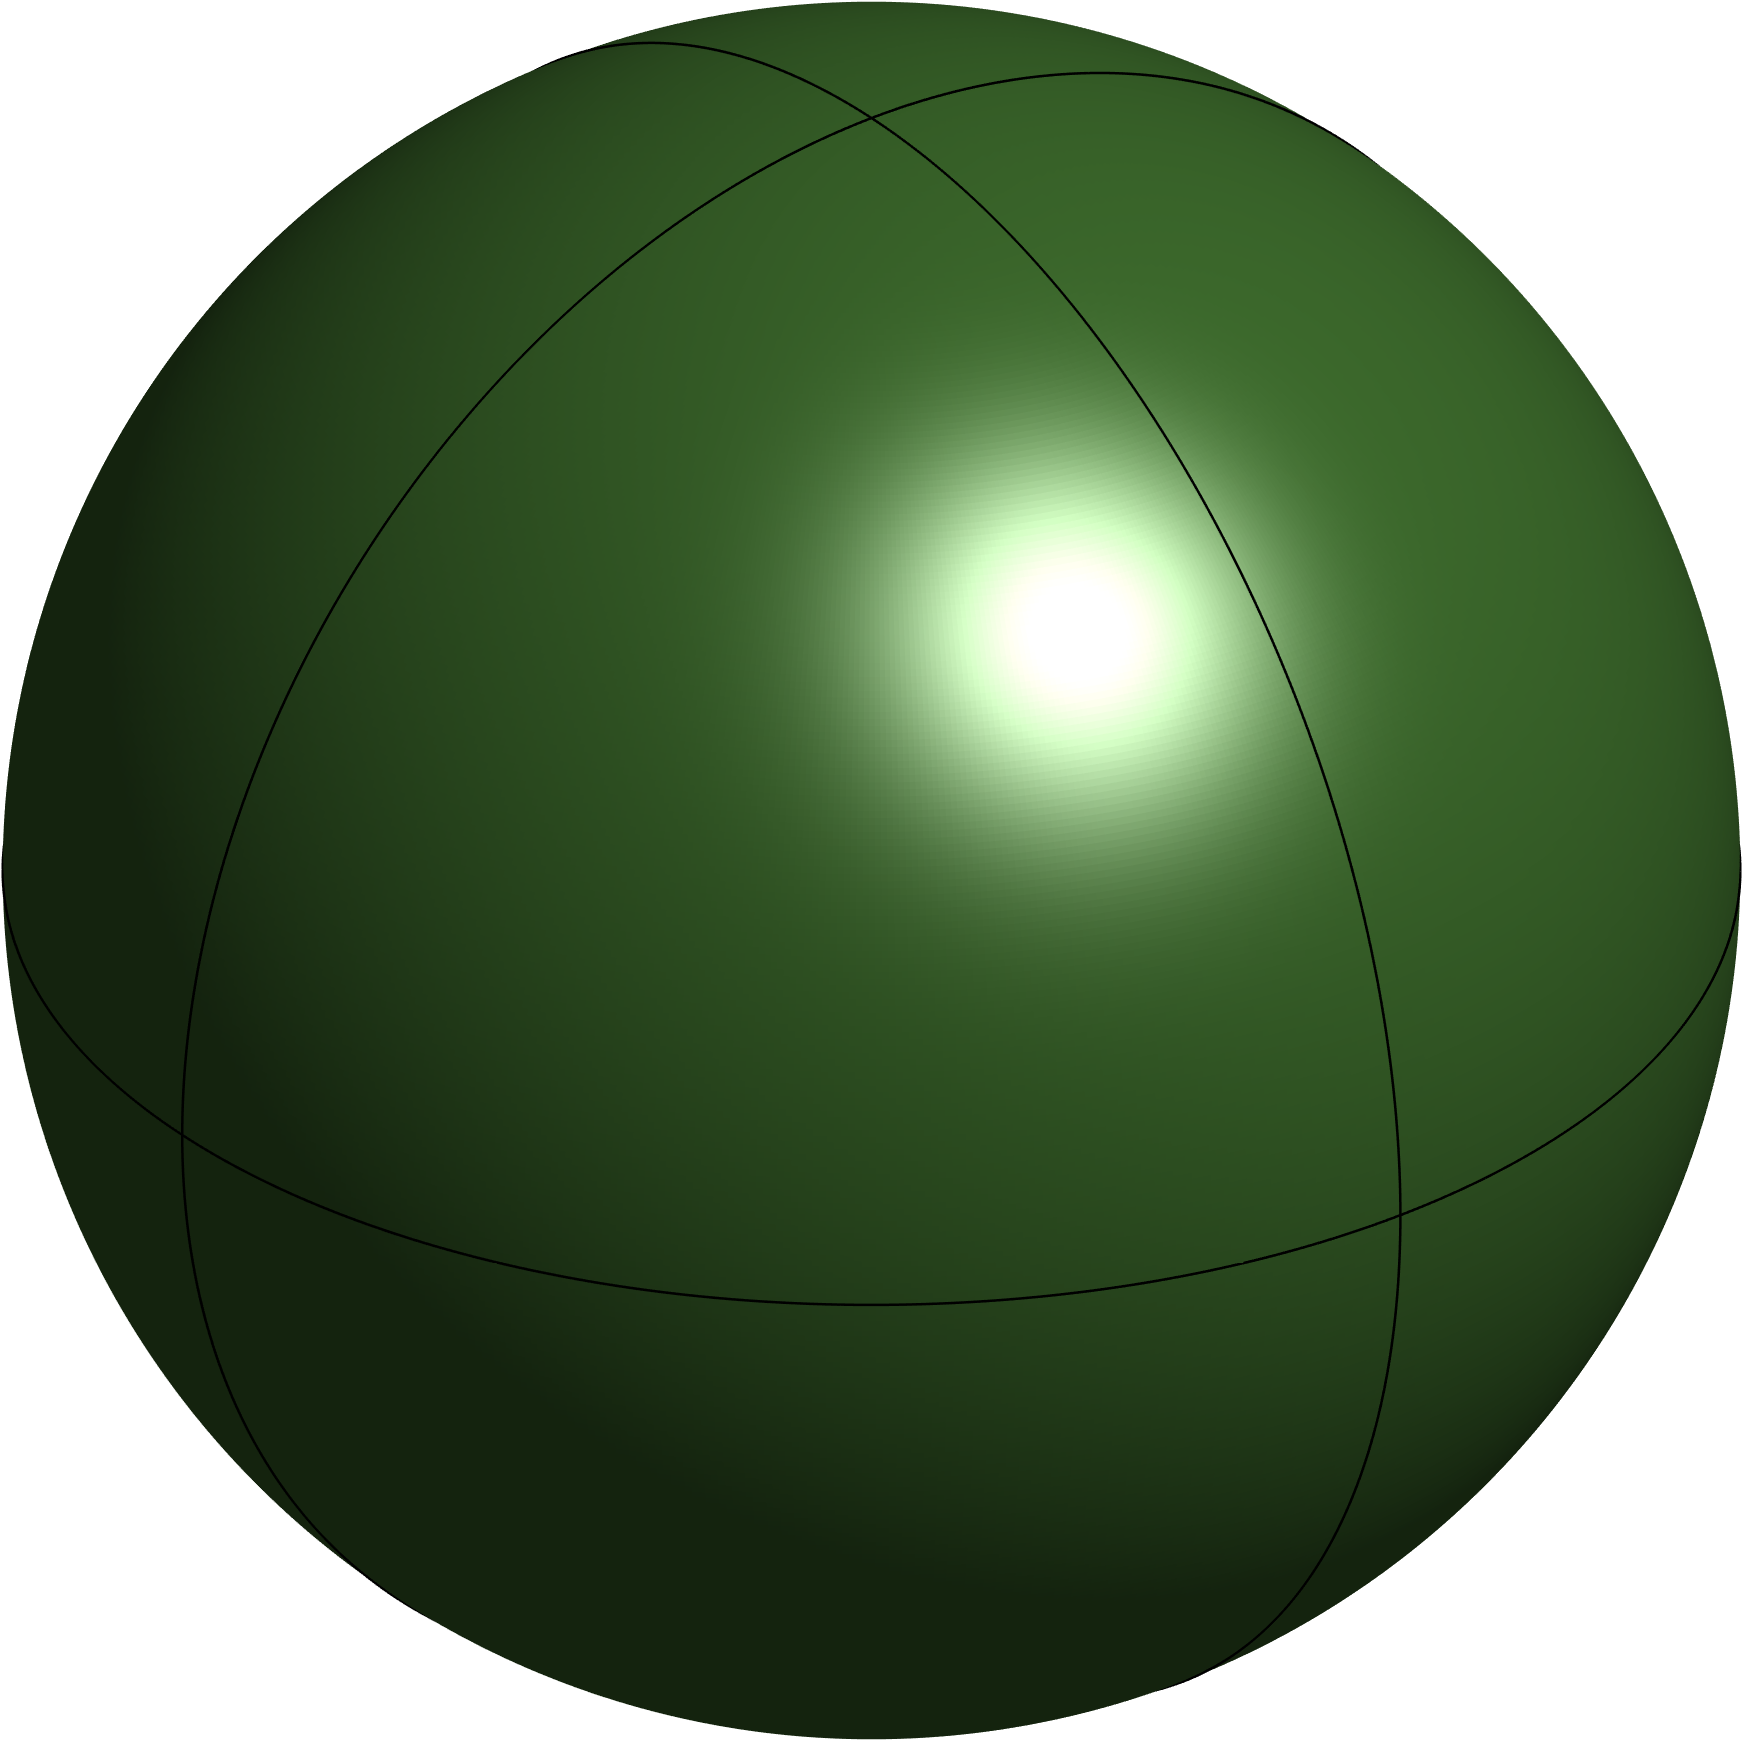
\includegraphics[width=0.8\textwidth]{../../graphics/sphericalShell/sphericalShellMesh1_2_0}
%		\includegraphics[width=0.8\textwidth]{\graphicsFolder/Figure5a}
		\caption{Mesh ${\cal M}_{1,\check{p},\check{k}}^{\textsc{iga}}$}
		\label{Fig2:SphericalShellMeshes1}
    \end{subfigure}
    ~
	\begin{subfigure}{0.3\textwidth}
		\centering
		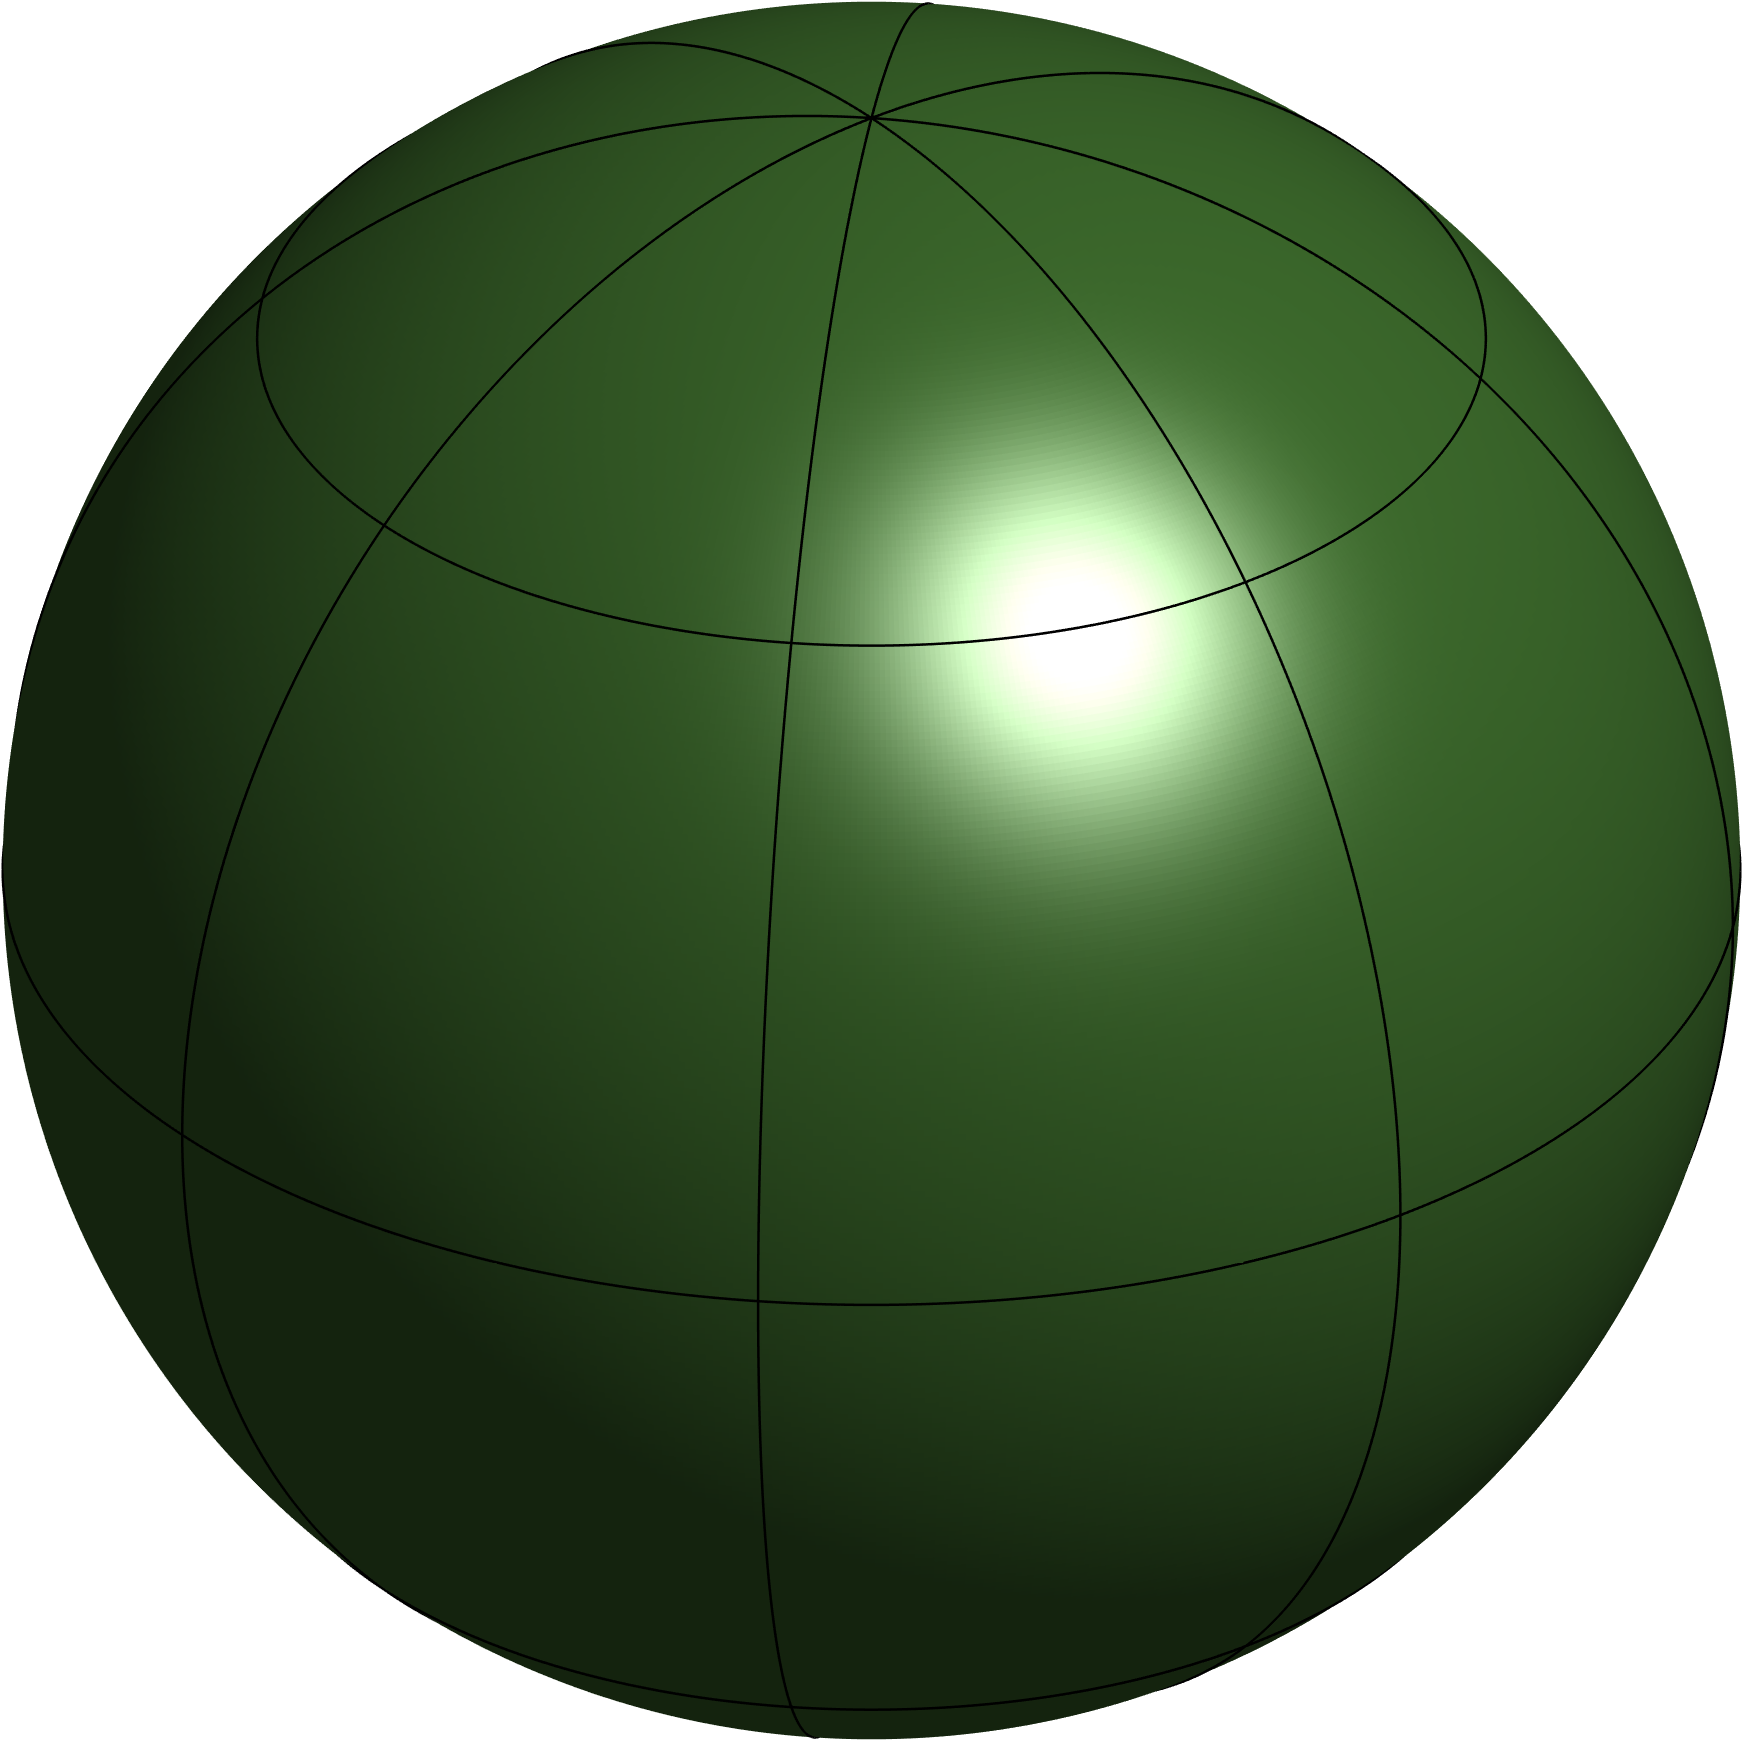
\includegraphics[width=0.8\textwidth]{../../graphics/sphericalShell/sphericalShellMesh2_2_0}
%		\includegraphics[width=0.8\textwidth]{\graphicsFolder/Figure5b}
		\caption{Mesh ${\cal M}_{2,\check{p},\check{k}}^{\textsc{iga}}$}
		\label{Fig2:SphericalShellMeshes2}
    \end{subfigure}
    ~
	\begin{subfigure}{0.3\textwidth}
		\centering
		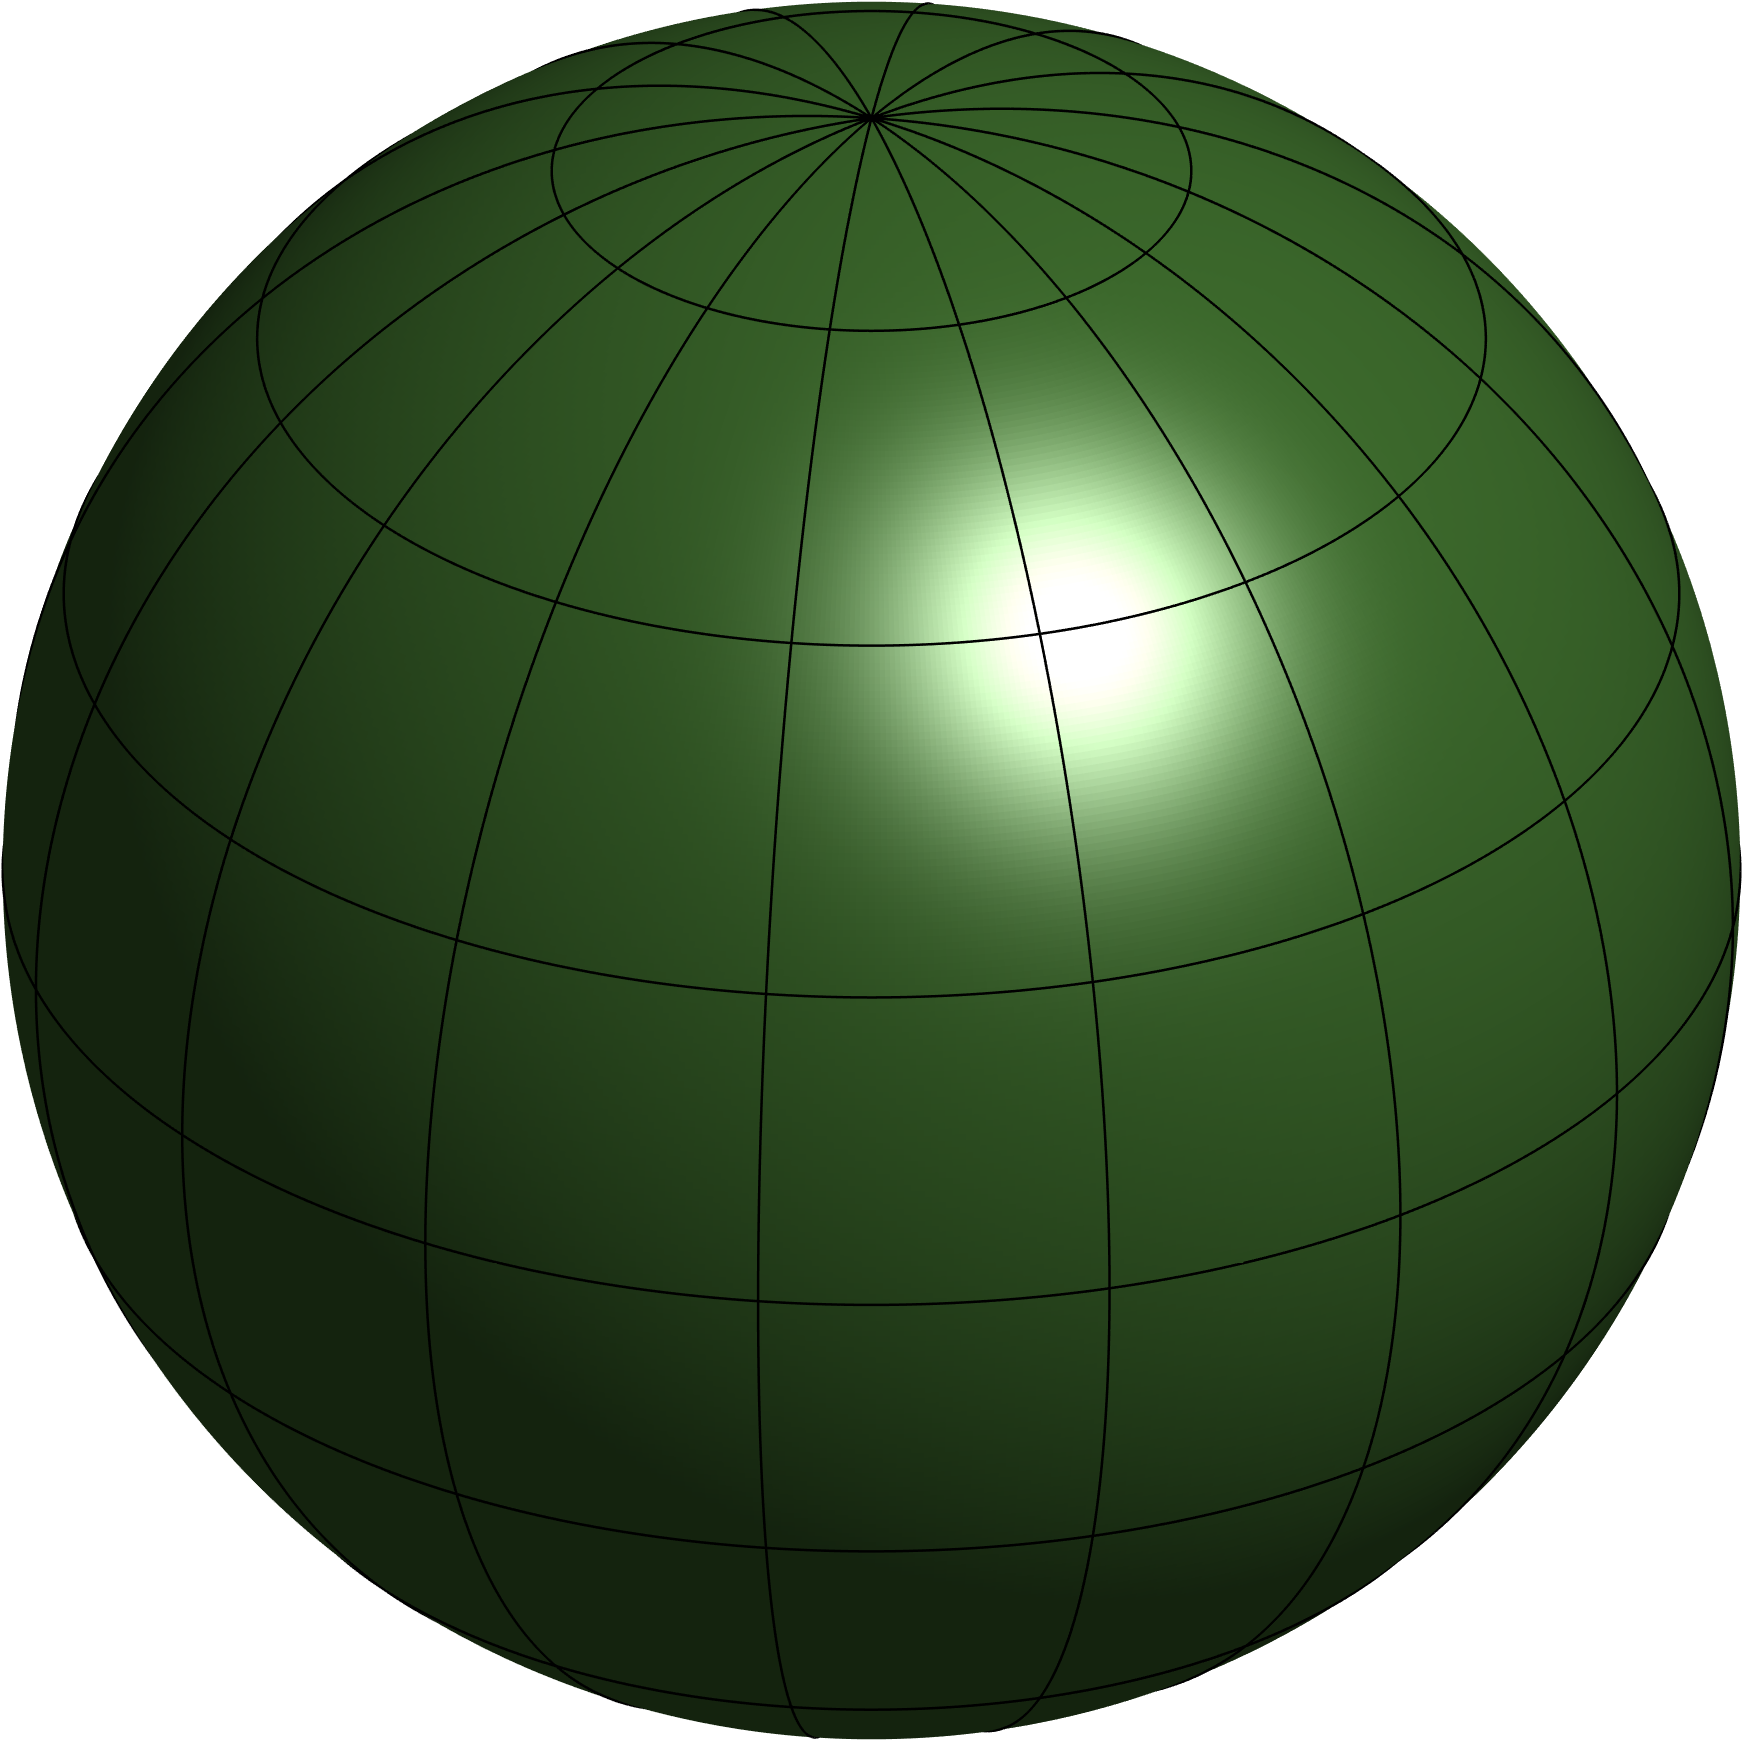
\includegraphics[width=0.8\textwidth]{../../graphics/sphericalShell/sphericalShellMesh3_2_0}
%		\includegraphics[width=0.8\textwidth]{\graphicsFolder/Figure5c}
		\caption{Mesh ${\cal M}_{3,\check{p},\check{k}}^{\textsc{iga}}$}
		\label{Fig2:SphericalShellMeshes3}
    \end{subfigure}
	\caption{\textbf{Numerical examples}: Illustration of the first three meshes, using two successive refinements from the coarse mesh ${\cal M}_{1,\check{p},\check{k}}^{\textsc{iga}}$.}
	\label{Fig2:SphericalShellMeshes}
\end{figure}

The meshes will be generated from a standard discretization of a sphere using NURBS as seen in \Cref{Fig2:SphericalShellMeshes}. We shall denote by ${\cal M}_{m,\check{p},\check{k}}^{\textsc{iga}}$, mesh number $m$ with polynomial order $\check{p}$ and continuity $\check{k}$ across element boundaries\footnote{Except for some possible $C^0$ lines in the initial CAD geometry.}. For the corresponding FEM meshes we denote by ${\cal M}_{m,\check{p},\mathrm{s}}^{\textsc{fem}}$ and ${\cal M}_{m,\check{p},\mathrm{i}}^{\textsc{fem}}$ the subparametric and isoparametric FEM meshes, respectively. The construction of NURBS meshes are illustrated in \Cref{Fig2:SphericalShellMeshes}. The initial mesh is depicted as mesh ${\cal M}_{1,\check{p},\check{k}}^{\textsc{iga}}$ in \Cref{Fig2:SphericalShellMeshes1} and is refined only in the angular directions for the first 3 refinements (that is, mesh ${\cal M}_{4,\check{p},\check{k}}^{\textsc{iga}}$ only have one element thickness in the radial direction). Mesh ${\cal M}_{m,\check{p},\check{k}}^{\textsc{iga}}$, $m=5,6,7$, have 2, 4 and 8 elements in its thickness, respectively. This is done to obtain low aspect ratios for the elements. All the meshes will then be nested and the refinements are done uniformly. We shall use the same polynomial order in all parameter directions; $\check{p}_\upxi=\check{p}_\upeta=\check{p}_\upzeta$. 

Unless otherwise stated, we shall use the BGU formulation and $N=4$ basis functions in the radial direction of the infinite elements.

\subsection{Simpson benchmark}
The configuration presented by Simpson et al.~\cite{Simpson2014aib} is considered: a rigid sphere of radius $R_0=\SI{0.5}{m}$ is impinged by an incident plane wave and the total pressure is measured at a distance $r=\SI{5}{m}$ from the origin. 

This is a low frequency problem with $k=\SI{2}{m^{-1}}$. It is emphasized that the trace of the NURBS discretization of the domain $\Omega_{\mathrm{a}}$ at the surface $\Gamma_0$ reduces to the exact same NURBS discretization used in~\cite{Simpson2014aib} to discretize the boundary $\Gamma_0$. 

From \Cref{Fig2:simpsonPlot} we observe that the IGA infinite element method (IGAIE) exploits the available degrees of freedom at $\Gamma_0$ more effectively than the IGA boundary element method (IGABEM) in~\cite{Simpson2014aib}\footnote{Due to low resolution of the plots in~\cite[Fig. 17]{Simpson2014aib}, the results were reproduced and sampled at 3601 points (rather than 30 points) using our own IGABEM implementation.}. 

By projecting the analytic solution onto this set of NURBS basis functions at $\Gamma_0$ (the best approximation in the $L_2$-norm by least squares projection, IGA best approximation, IGABA), it is revealed that even more accuracy can potentially be made. This is an inherent problem for Galerkin FEM when solving the Helmholtz equation and is related to the pollution effect \cite{Babuska1995agf}. All IEM formulations (PGU, PGC, BGU and BGC) gave approximately the same result in this case.
\begin{figure}
	\centering
	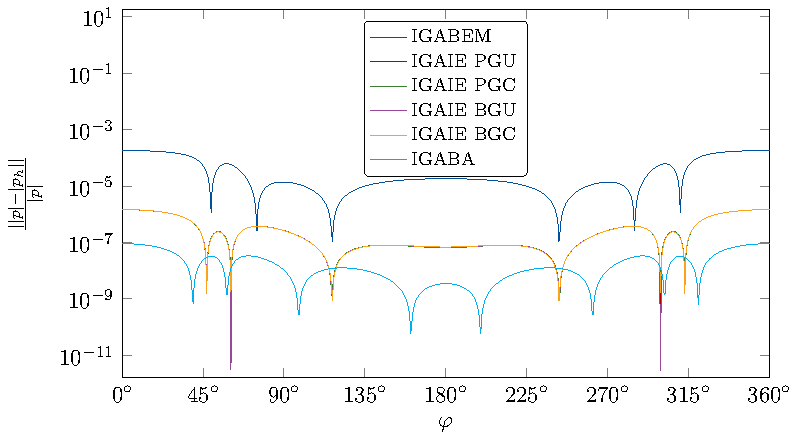
\includegraphics[width=\textwidth]{../../LaTeX/createFigures/TikzFigures/articleIGA_PhD/simpson}
%	\includegraphics[width=\textwidth]{\graphicsFolder/Figure6}
	\caption{\textbf{Simpson benchmark}: The relative error in the modulus of the pressure is plotted on a circle (azimuth direction, $\varphi$) in the $xy$-plane at $r=\SI{5}{m}$. All simulations were computed on mesh ${\cal M}_{3,3,2}^{\textsc{iga}}$. The IGAIE formulations here produce roughly the same result.}
	\label{Fig2:simpsonPlot}
\end{figure}

\subsection{Ihlenburg benchmark}
Three benchmark solutions based on the model problem after Ihlenburg~\cite[p. 191]{Ihlenburg1998fea} with parameters given in \Cref{Tab2:IhlenburgParameters}, are investigated. 
\begin{table}
	\centering
	\caption{\textbf{Ihlenburg benchmark}: Parameters for the Ihlenburg benchmark problems.}
	\label{Tab2:IhlenburgParameters}
	\begin{tabular}{l l}
		\toprule
		Parameter & Description\\
		\midrule
		$P_{\mathrm{inc}}=\SI{1}{Pa}$ & Amplitude of incident wave\\
		$E = \SI{2.07e11}{Pa}$ & Young's modulus\\
		$\nu = 0.3$ & Poisson's ratio\\
		$\rho_{\mathrm{s}} = \SI{7669}{kg.m^{-3}}$ & Density of solid\\
		$\rho_{\mathrm{f}} = \SI{1000}{kg.m^{-3}}$ & Density of water\\
		$c_{\mathrm{f}} = \SI{1524}{m.s^{-1}}$ & Speed of sound in water\\
		$R_0=\SI{5.075}{m}$ & Outer radius\\
		$R_1=\SI{4.925}{m}$ & Inner radius\\
		\bottomrule
	\end{tabular}
\end{table}
The parameters for the fluid domains are the speed of sound in water $c_{\mathrm{f}}$ and the fluid density $\rho_{\mathrm{f}}$, and the parameters for the solid domain are the Young's modulus, $E$, the Poisson's ratio $\nu$ and the solid density $\rho_{\mathrm{s}}$. The first benchmark is a simple rigid scattering case (with sound-hard boundary conditions, SHBC) on a sphere with radius $R_0$. The second benchmark problem on a spherical shell has ASI conditions at the outer radius, $R_0$, and homogeneous Neumann condition at the inner radius, $R_1$ (sound-soft boundary conditions, SSBC). This case can be thought of as an approximation of a scattering problem on a spherical shell with an internal fluid with very low density. The third and final benchmark is a further extension with ASI conditions on both sides of the spherical shell (Neumann-Neumann conditions on both surfaces of the shell, NNBC). All of these benchmarks have analytic solutions~\cite{Venas2019e3s} (see \Cref{Fig2:ihlenburgTSexact,Fig2:ihlenburg3Dexact}), which enables computation of the error in the energy norm. As we use the same parameters in both fluids, we denote the common wave number in these fluids by $k=k_1=k_2$.
\begin{figure}
	\centering
	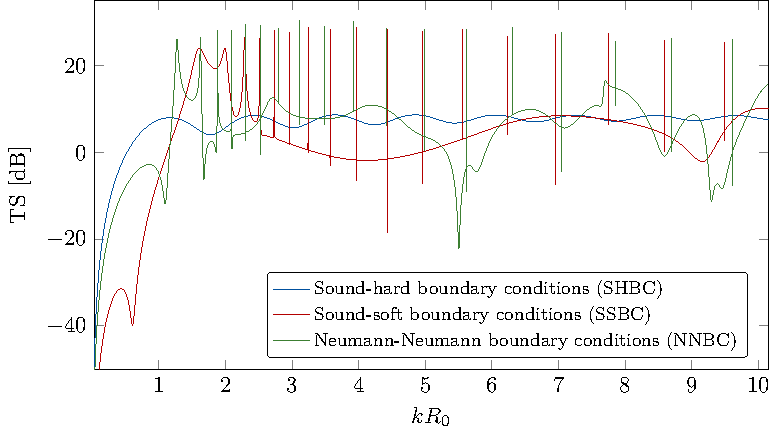
\includegraphics[width=\textwidth]{../../LaTeX/createFigures/TikzFigures/articleIGA_PhD/ihlenburg}
%	\includegraphics[width=\textwidth]{\graphicsFolder/Figure7}
	\caption{\textbf{Ihlenburg benchmark}: Analytic solutions to the scattering problem on a spherical shell with parameters given in \Cref{Tab2:IhlenburgParameters}. The far field pattern of backscattered pressure is plotted against the wave number $k$. A single Neumann condition at the outer radius, $R_0$, corresponds to the rigid scattering case with $\vec{u}=\zerovec$ and $p_2=0$. ASI at $R_0$ and Neumann at $R_1$ models $p_2=0$. Note that Ihlenburg~\cite[p. 192]{Ihlenburg1998fea} plots the far field pattern in \Cref{Eq2:farfield} instead of the target strength, $\TS$, in \Cref{Eq2:TS}.}
	\label{Fig2:ihlenburgTSexact}
\end{figure}
\begin{figure}
	\centering
	\begin{subfigure}[t]{0.48\textwidth}
		\centering
		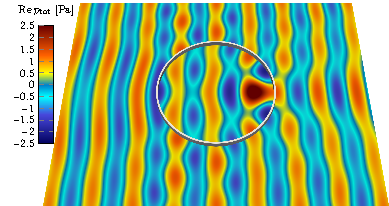
\includegraphics[width=\textwidth]{../../LaTeX/createFigures/TikzFigures/articleIGA_PhD/ihlenburg_nearField_real}
%		\includegraphics[width=\textwidth]{\graphicsFolder/Figure8a}
		\caption{Plot of the real part of the total pressure.}
	\end{subfigure}
	~
	\begin{subfigure}[t]{0.48\textwidth}
		\centering
		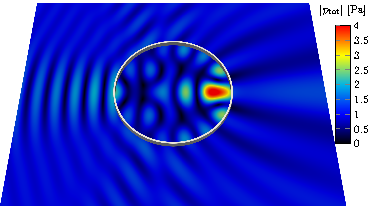
\includegraphics[width=\textwidth]{../../LaTeX/createFigures/TikzFigures/articleIGA_PhD/ihlenburg_nearField_abs}
%		\includegraphics[width=\textwidth]{\graphicsFolder/Figure8b}
		\caption{Plot of the modulus of the total pressure.}
	\end{subfigure}
	
	\caption{\textbf{Ihlenburg benchmark with NNBC}: The analytic solution with ASI at both $R_0$ and $R_1$ with $kR_0=10.15$ is plotted in the $xy$-plane. The solid domain is cut open for visualization purposes.}
	\label{Fig2:ihlenburg3Dexact}
\end{figure}
For each experiment, we use the same NURBS order everywhere. Denote by $\check{p}_\upxi = \check{p}_{\upxi,\mathrm{f}} = \check{p}_{\upxi,\mathrm{s}}$ the common NURBS order in the fluid and the solid in the $\xi$-direction. Similarly $\check{p}_\upeta = \check{p}_{\upeta,\mathrm{f}} = \check{p}_{\upeta,\mathrm{s}}$ and $\check{p}_\upzeta = \check{p}_{\upzeta,\mathrm{f}} = \check{p}_{\upzeta,\mathrm{s}}$. Moreover, we denote by $\check{p} = \check{p}_\upxi = \check{p}_\upeta = \check{p}_\upzeta$ the common polynomial orders in all domains.

In order to compare $C^0$ FEM and IGA on the scattering problem, we shall transform the NURBS mesh to a $C^0$ FEM mesh. We use the technique described in \Cref{Sec2:NURBStransformation} to get an isoparametric B-spline approximation of the geometry (isoparametric FEM). This parametrization will have $C^0$ continuity at element boundaries and correspondingly $G^0$ continuity of the geometry representation (i.e. with kinks). The geometric approximation error is of one order higher than the finite element approximation of the solution \cite{Strang1973aao}, so one could expect the $C^0$-IGA meshes (with $\check{k}=0$) to produce the same accuracy as the isoparametric FEM meshes of higher order ($\check{p}\geq 2$). It should be noted that the FEM analysis would then use the Bernstein basis instead of the classical Lagrange basis. However, both of these set of functions spans the same spaces, such that the results should be identical in the absence of round-off errors. 

In \Cref{Fig2:EnergyErrorPlotsDofs} we illustrate $h$-refinement through the error in the energy norm for the first benchmark example (rigid scattering).
\begin{figure}
	\centering
	\includegraphics[width=\textwidth]{../../LaTeX/createFigures/TikzFigures/articleIGA_PhD/L2normPlots_SHBC_dofs}
%	\includegraphics[width=\textwidth]{\graphicsFolder/Figure9}
	\caption{\textbf{Ihlenburg benchmark with SHBC}: Convergence analysis on the rigid scattering case with $k=\SI{1}{m^{-1}}$ and mesh ${\cal M}_m$, $m=1,\dots,7$, using $N=6$. The relative energy error (\Cref{Eq2:energyNormFluids}) is plotted against the degrees of freedom.}
	\label{Fig2:EnergyErrorPlotsDofs}
	\par\bigskip
	\includegraphics[width=\textwidth]{../../LaTeX/createFigures/TikzFigures/articleIGA_PhD/L2normPlots_SHBC_nepw}
%	\includegraphics[width=\textwidth]{\graphicsFolder/Figure10}
	\caption{\textbf{Ihlenburg benchmark with SHBC}: Convergence analysis on the rigid scattering case with $k=\SI{1}{m^{-1}}$ and mesh ${\cal M}_m$, $m=1,\dots,7$, using $N=6$. The relative energy error (\Cref{Eq2:energyNormFluids}) is plotted against the number of elements per wave.}
	\label{Fig2:EnergyErrorPlotsh}
\end{figure}
Predicted convergence rates are not obtained until the aspect ratio of the elements are reduced sufficiently (that is, from mesh ${\cal M}_4$ and onward). By comparing the results of mesh ${\cal M}_{m,2,\mathrm{i}}^{\textsc{fem}}$ and mesh ${\cal M}_{m,2,0}^{\textsc{iga}}$ it can be concluded that the geometry error of mesh ${\cal M}_{m,2,\mathrm{i}}^{\textsc{fem}}$ has almost no impact on the accuracy. However, when using maximum continuity, we get significantly better results. Expected convergence rates are visualized in \Cref{Fig2:EnergyErrorPlotsh} where we now plot the energy norm against $\lambda/h_{\mathrm{max}}$ (corresponding to the number of elements per wave) with $\lambda$ being the wavelength $\lambda=2\pi/k$. A key observation is that the number of elements per wave (needed to obtain a given accuracy) is greatly reduced with higher order IGA methods compared to the classical linear FEM (where 10 elements per wavelength is typically desired for engineering precision, \cite[p. 182]{Ihlenburg1998fea}). The result for the subparametric meshes ${\cal M}_{m,2,\mathrm{s}}^{\textsc{fem}}$ indicates that the convergence rate is reduced due to the reduced accuracy in the geometric representation. This is to be expected as shown in \cite[p. 202]{Strang1973aao}.

\begin{figure}
	\centering
	\begin{subfigure}{0.3\textwidth}
		\centering
		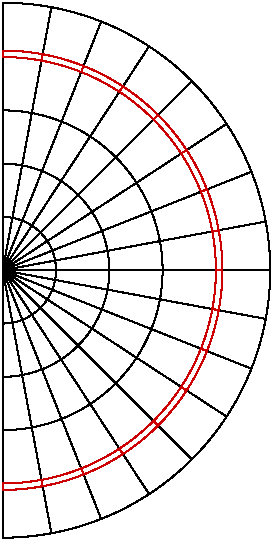
\includegraphics[width=0.6\textwidth]{../../graphics/sphericalShell/NNBC_IGAmesh4}
%		\includegraphics[width=0.6\textwidth]{\graphicsFolder/Figure11a}
		\caption{Mesh ${\cal M}_{4,\check{p},\check{k}}^{\textsc{iga}}$}
		\label{Fig2:SphericalShellMeshes1NNBC}
    \end{subfigure}
    ~
	\begin{subfigure}{0.3\textwidth}
		\centering
		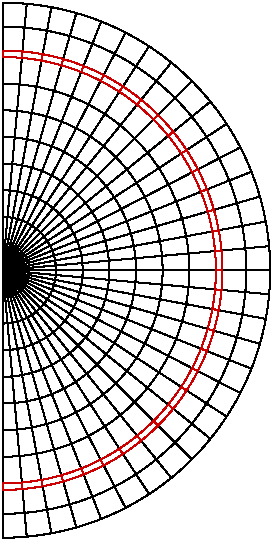
\includegraphics[width=0.6\textwidth]{../../graphics/sphericalShell/NNBC_IGAmesh5}
%		\includegraphics[width=0.6\textwidth]{\graphicsFolder/Figure11b}
		\caption{Mesh ${\cal M}_{5,\check{p},\check{k}}^{\textsc{iga}}$}
		\label{Fig2:SphericalShellMeshes2NNBC}
    \end{subfigure}
    ~
	\begin{subfigure}{0.3\textwidth}
		\centering
		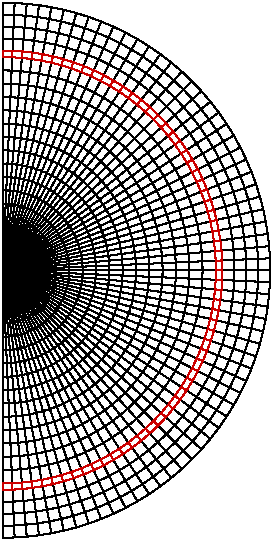
\includegraphics[width=0.6\textwidth]{../../graphics/sphericalShell/NNBC_FEMlinear6}
%		\includegraphics[width=0.6\textwidth]{\graphicsFolder/Figure11c}
		\caption{Mesh ${\cal M}_{6,1,\mathrm{i}}^{\textsc{fem}}$}
		\label{Fig2:SphericalShellMeshes3NNBC}
    \end{subfigure}
	\caption{\textbf{Ihlenburg benchmark with NNBC}: Illustration of some meshes for the full ASI problem in the $xz$-plane ($x>0$), where the mesh lines for the solid domain is colored red. The full mesh is obtained by rotation around the $z$-axis. Mesh ${\cal M}_{5,2,\mathrm{i}}^{\textsc{fem}}$ is visually indistinguishable from ${\cal M}_{5,\check{p},\check{k}}^{\textsc{iga}}$.}
	\label{Fig2:SphericalShellMeshesNNBC}
\end{figure}
Approaching the ASI problems, we illustrate some meshes in \Cref{Fig2:SphericalShellMeshesNNBC} for the full ASI problem. The corresponding meshes for the SSBC problem (with $p_2=0$) are obtained by removing the mesh inside the solid domain. In \Cref{Fig2:TSPlotSHBC,Fig2:errorPlotSHBC,Fig2:TSPlotSSBC,Fig2:errorPlotSSBC,Fig2:TSPlotNNBC,Fig2:errorPlotNNBC} the target strength, $\TS$, and the error in the energy norm is plotted against the scaled wave number, $kR_0$, in all of the three Ihlenburg benchmarks. As each frequency sweep is computed with a different number of degrees of freedom, one should draw the conclusions based on comparing both the accuracy of the results and the related computational costs.

Some data from simulations at $k=\SI{1}{m^{-1}}$ are reported in \Cref{Tab2:dataRigidScattering} (simulation run with 12 processors of the type Intel(R) Xeon(R) CPU E5-4650 2.70GHz). It should be noted that all simulations were done using the same code, such that the computational time for the FEM simulations can be optimized. However, this is actually the case for the IGA code as well since the implementation does not utilize optimized quadrature rules. The integration is done with $(\check{p}+1)^3$ quadrature points per element when building the system. For higher order splines spaces this is significantly more quadrature point than what is needed for exact integration (on meshes with affine geometry mapping\footnote{Using the same quadrature scheme on truly isoparametric elements will according to \cite[p. 256]{Ciarlet1991bee} give a numerical integration error of the same order as the finite element discretization error. Thus, the argument for optimal quadrature scheme also holds for isoparametric elements as well.}). In \cite{Hughes2010eqf,Johannessen2017oqf}, it is shown that the optimal number of quadrature points is half the number of degrees of freedom of the splines space under consideration. That is, the number of quadrature points in the IGA 3D tensor product meshes can be reduced by a factor up to $2^3(\check{p}+1)^3$ for meshes with maximal continuity. Thus, the efficiency of the IGA simulation may be improved significantly.

A particular interesting observation is that IGA obtains roughly the same accuracy as FEM when the same number of elements is used, even though this corresponds to far less degrees of freedom for the IGA simulation. Moreover, even better result can be obtained with less degrees of freedom if the polynomial degree is increased in the IGA simulations. This, however, only occurs when the mesh resolves the number of waves per element. When the mesh is sufficiently resolved, one order of magnitude improvement in the accuracy is obtained by increasing the polynomial degree. Since another magnitude of accuracy is obtained by using higher order elements in FEM/IGA, the IGA offers several orders of magnitude better accuracy than classical linear FEM. 

The peaks in the frequency sweeps represent eigenmodes. The quality of the numerical approximation of the corresponding frequencies is reduced for higher frequencies, resulting in fictitious modes. This typically does not pose that much of a problem as the bandwidth of these eigenmodes becomes very small, with a corresponding reduction in the energy they represent. Note that mesh ${\cal M}_{4,3,2}^{\textsc{iga}}$ performs particularly poorly on the partial ASI problem due to a fictitious mode at $k=\SI{1}{m^{-1}}$ for this mesh. The improvement offered by IGA concerning the accuracy in the eigenmodes is investigated in~\cite{Venas2015iao}. 

It should be noted that the meshes used throughout this work are not optimal. This is in particular the case for the full ASI problem where the density of elements becomes large at the origin. These meshes were used as they naturally arise from tensor product NURBS meshes of spherical shells and spheres. One could thus obtain increased performance for the FEM solutions using standard meshing of the domain. However, locally refined meshes can also be obtained with the IGA method, for example using LR B-splines \cite{Johannessen2014iau}.

\begin{table}
	\centering
	\caption{\textbf{Ihlenburg benchmark}: Data for some simulations on the rigid scattering problem with $k=\SI{1}{m^{-1}}$. The errors are given in the energy norm (\Cref{Eq2:energyNorm}). For each simulation, the mesh number, the polynomial order, $\check{p}$, the number of mesh elements $n_{\mathrm{el}}$ (not including the infinite elements) and the number of degrees of freedom $n_{\mathrm{dof}}$, is reported. The elapsed times for building the system $t_{\mathrm{sys}}$ and for solving the system $t_{\mathrm{sol}}$ (using LU-factorization) are also included (times in seconds). Finally, the relative error in the energy norm is given in percentage.}
	\label{Tab2:dataRigidScattering}
	\begin{subtable}[t]{\linewidth}
		\caption{Sound-hard boundary conditions (SHBC).}
		\label{Tab2:dataRigidScatteringSHBC}
		\centering
		\bgroup
		\def\arraystretch{1.1}%
		\begin{tabular}{l S[table-format = 6.0] S[table-format = 5.0] S[table-format = 2.1,round-mode=places,round-precision=1] S[table-format = 2.1,round-mode=places,round-precision=1] S[table-format = 1.2]}
			\hline
			 		   & {$n_{\mathrm{el}}$} & {$n_{\mathrm{dof}}$} &{$t_{\mathrm{sys}}$ [s]}	& {$t_{\mathrm{sol}}$ [s]} 		& {Relative energy error [\%]} \\
			\hline
			Mesh ${\cal M}_{6,1,\mathrm{i}}^{\textsc{fem}}$		& 32768	& 56462	& 7.70	& 26.50	& 5.04	\cr
Mesh ${\cal M}_{5,2,\mathrm{i}}^{\textsc{fem}}$		& 4096	& 56462	& 5.07	& 20.48	& 0.62	\cr
Mesh ${\cal M}_{5,2,1}^{\textsc{iga}}$				& 4096	& 13476	& 4.79	& 4.32	& 0.64	\cr
Mesh ${\cal M}_{4,3,2}^{\textsc{iga}}$				& 512	& 4572	& 3.06	& 1.64	& 0.38	\cr
Mesh ${\cal M}_{5,3,2}^{\textsc{iga}}$				& 4096	& 17654	& 14.75	& 8.30	& 0.05	\cr

			\hline
		\end{tabular}
		\egroup
	\end{subtable}
	\par\bigskip
	\begin{subtable}[t]{\linewidth}
		\caption{Sound-soft boundary conditions (SSBC).}
		\label{Tab2:dataRigidScatteringSSBC}
		\centering
		\bgroup
		\def\arraystretch{1.1}%
		\begin{tabular}{l S[table-format = 6.0] S[table-format = 6.0] S[table-format = 2.1,round-mode=places,round-precision=1] S[table-format = 3.1,round-mode=places,round-precision=1] S[table-format = 2.2]}
			\hline
			 		   & {$n_{\mathrm{el}}$} & {$n_{\mathrm{dof}}$} &{$t_{\mathrm{sys}}$ [s]}	& {$t_{\mathrm{sol}}$ [s]} 		& {Relative energy error [\%]} \\
			\hline
			Mesh ${\cal M}_{6,1,\mathrm{i}}^{\textsc{fem}}$		& 40960	& 104858	& 13.66	& 75.28	& 7.66	\cr
Mesh ${\cal M}_{5,2,\mathrm{i}}^{\textsc{fem}}$		& 6144	& 129056	& 15.85	& 106.07	& 1.35	\cr
Mesh ${\cal M}_{5,2,1}^{\textsc{iga}}$				& 6144	& 33690	& 13.35	& 34.68	& 0.99	\cr
Mesh ${\cal M}_{4,3,2}^{\textsc{iga}}$				& 1024	& 13716	& 11.83	& 9.04	& 41.30	\cr
Mesh ${\cal M}_{5,3,2}^{\textsc{iga}}$				& 6144	& 47918	& 52.03	& 69.94	& 0.09	\cr

		    \hline
		\end{tabular}
		\egroup
	\end{subtable}	
	\par\bigskip
	\begin{subtable}[t]{\linewidth}
		\caption{Neumann-Neumann boundary conditions (NNBC).}
		\label{Tab2:dataRigidScatteringNNBC}
		\centering
		\bgroup
		\def\arraystretch{1.1}%
		\begin{tabular}{l S[table-format = 6.0] S[table-format = 6.0] S[table-format = 2.1,round-mode=places,round-precision=1] S[table-format = 3.1,round-mode=places,round-precision=1] S[table-format = 1.2]}
			\hline
			 		  & {$n_{\mathrm{el}}$} & {$n_{\mathrm{dof}}$} &{$t_{\mathrm{sys}}$ [s]}	& {$t_{\mathrm{sol}}$ [s]} 		& {Relative energy error [\%]} \\
			\hline
			Mesh ${\cal M}_{6,1,\mathrm{i}}^{\textsc{fem}}$		& 172032	& 233915	& 27.80	& 429.52	& 6.55	\cr
Mesh ${\cal M}_{5,2,\mathrm{i}}^{\textsc{fem}}$		& 22528	& 258113	& 31.05	& 462.66	& 0.53	\cr
Mesh ${\cal M}_{5,2,1}^{\textsc{iga}}$				& 22528	& 53905	& 22.46	& 64.91	& 0.71	\cr
Mesh ${\cal M}_{4,3,2}^{\textsc{iga}}$				& 3072	& 18289	& 17.10	& 17.28	& 1.47	\cr
Mesh ${\cal M}_{5,3,2}^{\textsc{iga}}$				& 22528	& 73139	& 93.22	& 145.74	& 0.05	\cr

		    \hline
		\end{tabular}
		\egroup
	\end{subtable}	
\end{table}

\begin{figure}
	\centering
	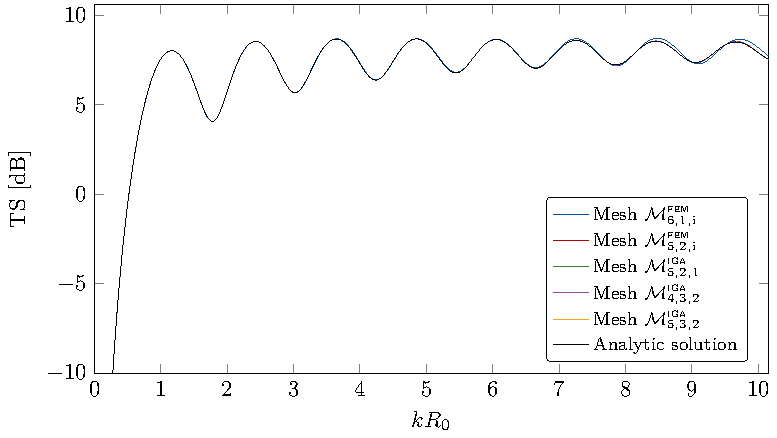
\includegraphics[width=\textwidth]{../../LaTeX/createFigures/TikzFigures/articleIGA_PhD/ihlenburg_farField_TSPlotSHBC}
%	\includegraphics[width=\textwidth]{\graphicsFolder/Figure12}
	\caption{\textbf{Ihlenburg benchmark with SHBC}: The target strength (TS) in \Cref{Eq2:TS} is plotted against $kR_0$.}
	\label{Fig2:TSPlotSHBC}
	\par\bigskip
	\par\bigskip
	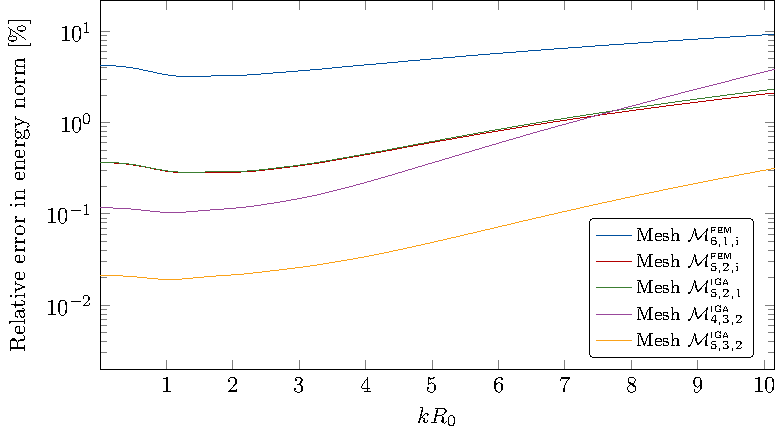
\includegraphics[width=\textwidth]{../../LaTeX/createFigures/TikzFigures/articleIGA_PhD/ihlenburg_farField_errorPlotSHBC}
%	\includegraphics[width=\textwidth]{\graphicsFolder/Figure13}
	\caption{\textbf{Ihlenburg benchmark with SHBC}: The relative energy norm (\Cref{Eq2:energyNorm}) is plotted against $kR_0$.}
	\label{Fig2:errorPlotSHBC}
\end{figure}
\begin{figure}
	\centering
	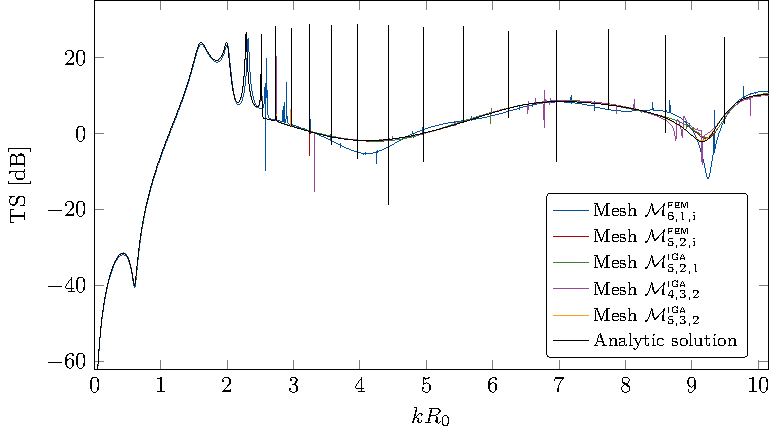
\includegraphics[width=\textwidth]{../../LaTeX/createFigures/TikzFigures/articleIGA_PhD/ihlenburg_farField_TSPlotSSBC}
%	\includegraphics[width=\textwidth]{\graphicsFolder/Figure14}
	\caption{\textbf{Ihlenburg benchmark with SSBC}: ASI problem with the internal pressure modeled to be $p_2=0$. The target strength (TS) in \Cref{Eq2:TS} is plotted against $kR_0$.}
	\label{Fig2:TSPlotSSBC}
	\par\bigskip
	\par\bigskip
	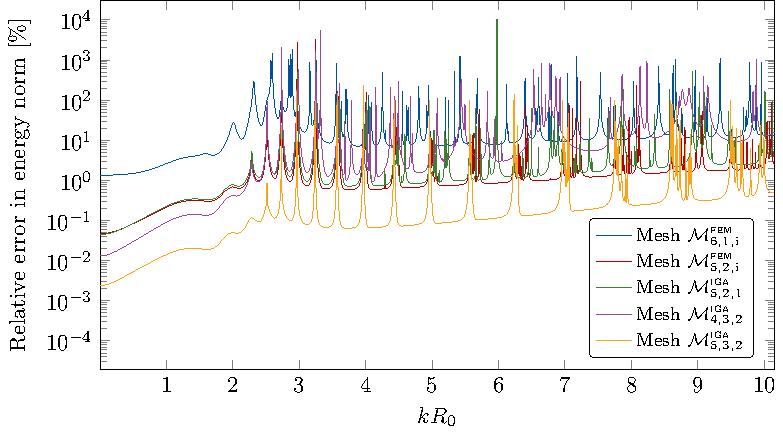
\includegraphics[width=\textwidth]{../../LaTeX/createFigures/TikzFigures/articleIGA_PhD/ihlenburg_farField_errorPlotSSBC}
%	\includegraphics[width=\textwidth]{\graphicsFolder/Figure15}
	\caption{\textbf{Ihlenburg benchmark with SSBC}: ASI problem with the internal pressure modeled to be $p_2=0$. The relative energy norm (\Cref{Eq2:energyNorm}) is plotted against $kR_0$.}
	\label{Fig2:errorPlotSSBC}
\end{figure}
\begin{figure}
	\centering
	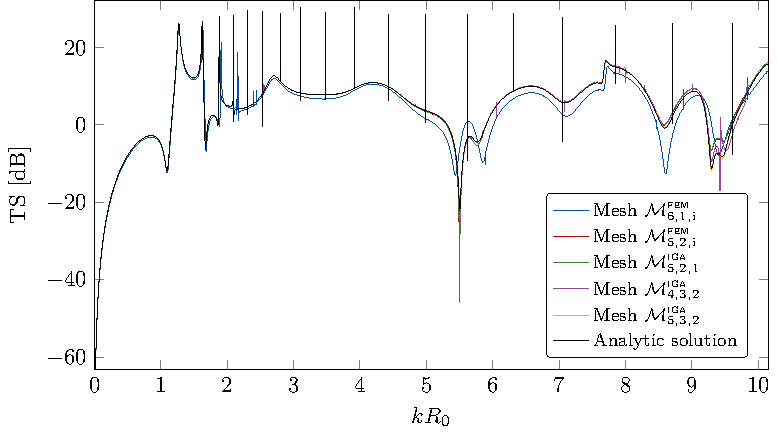
\includegraphics[width=\textwidth]{../../LaTeX/createFigures/TikzFigures/articleIGA_PhD/ihlenburg_farField_TSPlotNNBC}
%	\includegraphics[width=\textwidth]{\graphicsFolder/Figure16}
	\caption{\textbf{Ihlenburg benchmark with NNBC}: The target strength (TS) in \Cref{Eq2:TS} is plotted against $kR_0$.}
	\label{Fig2:TSPlotNNBC}
	\par\bigskip
	\par\bigskip
	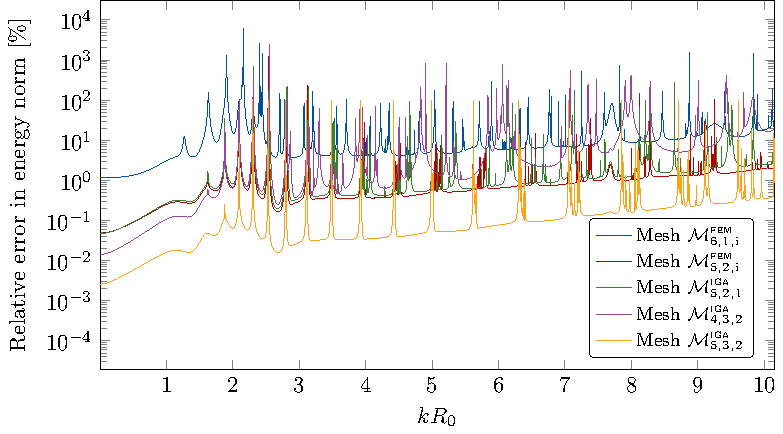
\includegraphics[width=\textwidth]{../../LaTeX/createFigures/TikzFigures/articleIGA_PhD/ihlenburg_farField_errorPlotNNBC}
%	\includegraphics[width=\textwidth]{\graphicsFolder/Figure17}
	\caption{\textbf{Ihlenburg benchmark with NNBC}: The relative energy norm (\Cref{Eq2:energyNorm}) is plotted against $kR_0$.}
	\label{Fig2:errorPlotNNBC}
\end{figure}
In \Cref{Fig2:energyErrorPlot} we visualize the distribution of the error of the full ASI problem. The error is observed to be largest at element boundaries where the continuity is reduced. Since second order basis functions are used and the error in the velocity/stress dominates the error in the pressure/displacement, the results are in agreement with what was observed in \cite{Kumar2017spr}, i.e., that the error in the derivative of the primary solution is largest at the element boundaries.
\begin{figure}
	\centering
	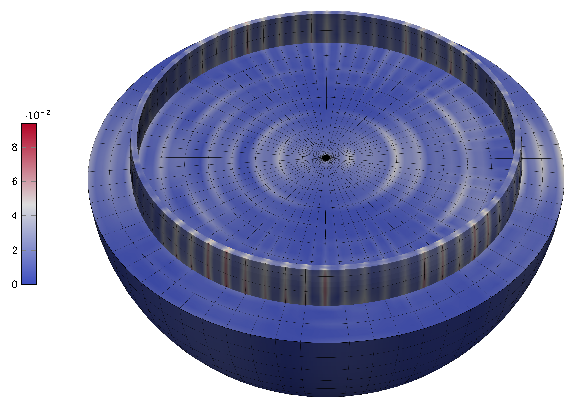
\includegraphics[width=0.7\textwidth]{../../LaTeX/createFigures/TikzFigures/articleIGA_PhD/energyErrorPlot}
%	\includegraphics[width=0.7\textwidth]{\graphicsFolder/Figure18}
	\caption{\textbf{Ihlenburg benchmark with NNBC}: Simulation of the full ASI problem on mesh ${\cal M}_{5,2,1}^{\textsc{iga}}$. Pointwise evaluation of the square root of the integrand of the volume integrals in the energy norm $\energyNorm{U-U_h}{\Omega}$ in \Cref{Eq2:energyNorm} with $k=\SI{2}{m^{-1}}$ (error in the infinite elements in $\Omega_{\mathrm{a}}^+$ is not shown) is here visualized, where $U$ is the set of analytic solutions in both fluid domains and the solid domain, and $U_h$ is the corresponding numerical solution. The values are scaled by the square root of the maximum of the corresponding integrand values of $\energyNorm{U}{\Omega}$. Both fluid domains are cut open at the $xy$-plane (at $z=0$), and the solid domain is cut open at $z=\SI{1.1}{m}$.}
	\label{Fig2:energyErrorPlot}
\end{figure}

\subsection{Radial pulsation from a mock shell}
\label{Subsec2:mockShell}
By construction of the fundamental solution of the Helmholtz equation ($\Phi_k(\vec{x},\vec{y})$ in \Cref{Eq2:FreeSpaceGrensFunction}), the function $p(\vec{x}) = \Phi_k(\vec{x},\vec{y})$ is a solution to \Cref{Eq2:HelmholtzEqn,Eq2:HelmholtzEqnNeumannCond,Eq2:sommerfeldCond} whenever $\vec{y}\in\R^3\setminus\overline{\Omega^+}$ and for the Neumann boundary condition $g(\vec{x})=\partial_n\Phi_k(\vec{x},\vec{y})$ on $\Gamma_0$.  Hence, we have an exact reference solution for the exterior Helmholtz problem for arbitrary geometries $\Gamma_0$ which encloses the point $\vec{y}$. It is emphasized that this solution is non-physical for non-spherical geometries $\Gamma_0$. General solutions may be constructed by separation of variables (cf.~\cite[p. 26]{Ihlenburg1998fea})
\begin{equation}
	p(\vec{x}) = \sum_{n=0}^\infty\sum_{m=-n}^n C_{nm} \hankel_n^{(1)}(kR) \legendre_n^{|m|}(\cos\vartheta)\euler^{\imag m\varphi} 
\end{equation}
with
\begin{equation*}
	R = |\vec{x}-\vec{y}|,\quad \vartheta=\arccos\left(\frac{x_3-y_3}{R}\right),\quad\varphi = \operatorname{atan2}(x_2-y_2,x_1-y_1)
\end{equation*}
where $\hankel_n^{(1)}$ is the $n^{\mathrm{th}}$ spherical Hankel function of first kind and $\legendre_n^m$ are the associated Legendre functions. In fact, the solution $p(\vec{x}) = \Phi_k(\vec{x},\vec{y})$ is a special case of this general form with 
\begin{equation}
	C_{nm} = \begin{cases}
		\frac{\imag k}{4\PI} & n = 0,\,\,m=0\\
		0 & \text{otherwise}.
		\end{cases}
\end{equation}
The complexity of this problem setup does not scale with the complexity of the model as it is independent of $\Gamma_0$. However, it preserves two important properties of acoustic scattering, namely the radial decay and the oscillatory nature. Thus, this problem setup represents a general way of constructing manufactured solutions, that can be utilized to verify the correctness of the implemented code for solving the Helmholtz equation. A special case of this general setup is the pulsating sphere example in~\cite{Simpson2014aib}.

From the first limit of \Cref{Eq2:Phi_k_limits1,Eq2:Phi_k_limits2}, the far field is given by $p_0(\hat{\vec{x}})=\frac{1}{4\PI}\euler^{-\imag k \hat{\vec{x}}\cdot\vec{y}}$. Thus, the target strength is a constant, $\TS=-20\log_{10}(4\PI)\approx -21.984$ (where we define $P_{\mathrm{inc}}=\SI{1}{Pa}$ in \Cref{Eq2:TS} for this problem). 

Consider the case $\vec{y}=\frac{R_0}{4}(1,1,1)$ and the boundary $\Gamma_0$ given by a \textit{mock shell} composed of a cylinder with hemispherical endcaps (with axis of symmetry along the $x$-axis such that the center of the spherical endcaps are located at $x = 0$ and $x = -L$). The cylinder has radius $R_0=\SI{1}{m}$ and length $L=\frac{\PI}{2}R_0$. The analytic solution is given by
\begin{equation}
	p(\vec{x}) = \frac{\euler^{\imag kR}}{4\PI R},\quad R=|\vec{x}-\vec{y}|
\end{equation}
and the Neumann condition is then
\begin{equation}
	g(\vec{x}) = \frac{\euler^{\imag kR}}{4\PI R^3}(\imag kR -1) (\vec{x}-\vec{y})\cdot\vec{n}(\vec{x}).
\end{equation}

This example is used to illustrate the differences of the infinite element formulations using the prolate ellipsoidal elements after Burnett~\cite{Burnett1994atd}. The mesh construction is illustrated in \Cref{Fig2:MS_meshes}, and an illustration of the solution is presented in \Cref{Fig2:MS_visualization}.
\begin{figure}
	\centering    
	\begin{subfigure}{0.49\textwidth}
		\centering
%		\includegraphics[width=\textwidth]{\graphicsFolder/Figure19a}
		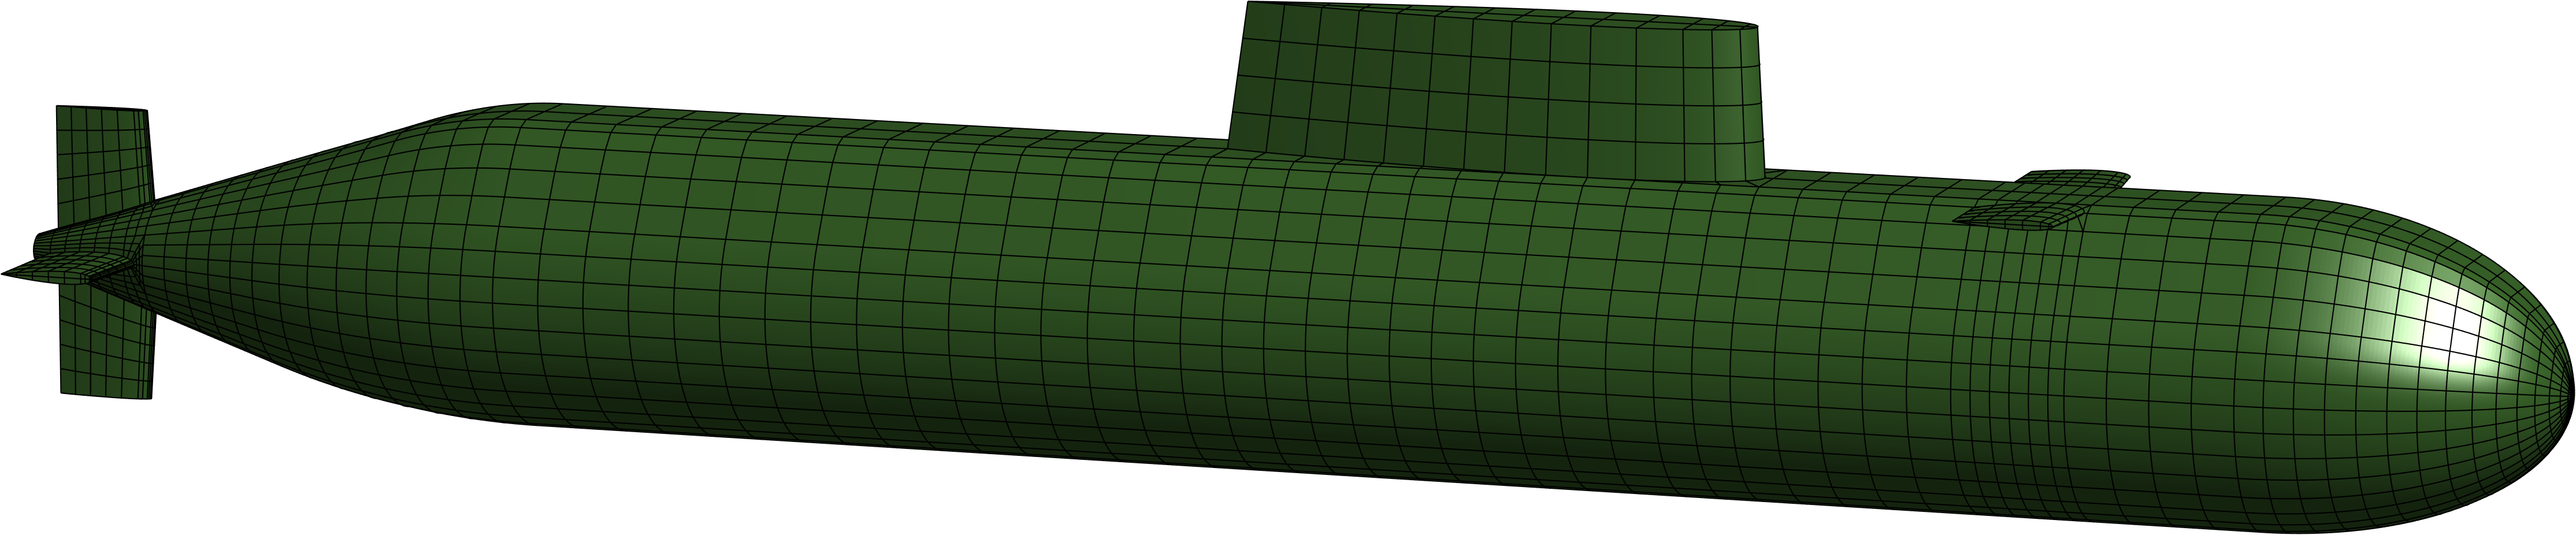
\includegraphics[width=\textwidth]{../../graphics/MS_P/mesh1}
		\caption{Mesh 1.}
	\end{subfigure}%
	\hspace*{0.02\textwidth}%
	\begin{subfigure}{0.49\textwidth}
%		\includegraphics[width=\textwidth]{\graphicsFolder/Figure19b}
		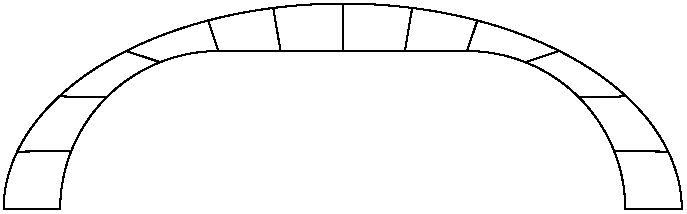
\includegraphics[width=\textwidth]{../../graphics/MS_P/mesh3}
		\caption{Mesh 3.}
	\end{subfigure}
	\par\bigskip
	\begin{subfigure}{0.49\textwidth}
		\centering
%		\includegraphics[width=\textwidth]{\graphicsFolder/Figure19c}
		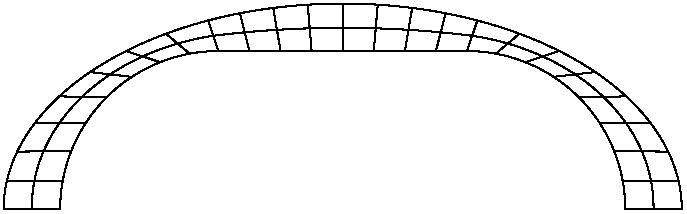
\includegraphics[width=\textwidth]{../../graphics/MS_P/mesh4}
		\caption{Mesh 4.}
	\end{subfigure}%
	\hspace*{0.02\textwidth}%
	\begin{subfigure}{0.49\textwidth}
%		\includegraphics[width=\textwidth]{\graphicsFolder/Figure19d}
		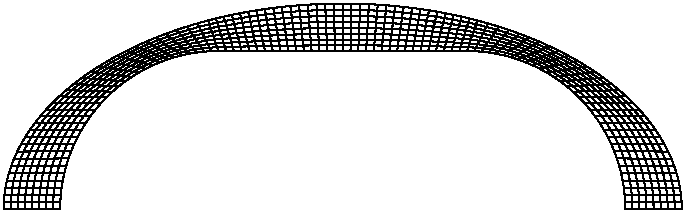
\includegraphics[width=\textwidth]{../../graphics/MS_P/mesh6}
		\caption{Mesh 6.}
	\end{subfigure}
	\caption{\textbf{Radial pulsation from a mock shell}: Meshes for the fluid domain between the scatterer and the artificial boundary. The meshes are constructed from the initial mesh 1, which is rotated around the axis of symmetry using four elements. Mesh 2 and 3 are refined only in the angular direction, while the more refined meshes also refine in the radial direction to obtain smallest aspect ratio. The meshes are nested.}
	\label{Fig2:MS_meshes}
\end{figure}
\begin{figure}
	\centering
%	\includegraphics[width=\textwidth]{\graphicsFolder/Figure20}
	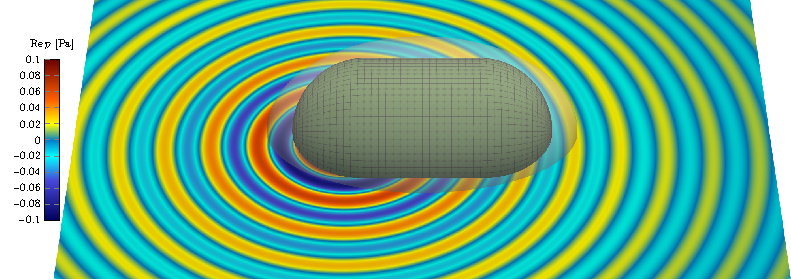
\includegraphics[width=\textwidth]{../../LaTeX/createFigures/TikzFigures/articleIGA_PhD/MS_PnearField}
	\caption{\textbf{Radial pulsation from a mock shell}: Visualization of numerical solution in the $xy$-plane using BGU with $N=6$ on mesh 5.}
	\label{Fig2:MS_visualization}
\end{figure}
Convergence plots are shown in \Cref{Fig2:MS_convergence}. Gerdes did a similar comparison in~\cite{Gerdes1998tcv} where scattering on a sphere was investigated. Our results verify these findings, namely lower errors for the unconjugated formulations (cf. \Cref{Fig2:MS_convergence}). Good results can be obtained using only a single radial shape function in case of unconjugated formulations. For the conjugated versions, on the other hand, $N > 6$ functions are needed to obtain similar accuracy and more degrees of freedom are required to get an asymptotic behavior.

In \Cref{Fig2:MS_condNumbersB} and \Cref{Fig2:MS_condNumbersP} the condition number is investigated for the different formulations and basis functions in the radial shape functions. The condition number for the unconjugated versions increases more rapidly as a function of $N$ compared to the corresponding formulations in the conjugated case. The condition number of the Lagrange basis increases particularly fast with $N$, making it useless\footnote{In the case of $r_n = nr_{\mathrm{a}}$.} for the conjugated formulations. However, the Lagrange basis yields the best result for the unconjugated formulations for small $N$. The Chebyshev basis seems to give the best condition numbers for the conjugated formulations for large $N$ (which is required for acceptable results). The unconjugated formulations perform quite similar, both in terms of the condition numbers and the error. The BGU formulation has the additional advantage of producing symmetric matrices and reduces the memory requirement. 
\begin{figure}
	\centering    
	\begin{subfigure}{0.49\textwidth}
		\centering
%		\includegraphics[width=\textwidth]{\graphicsFolder/Figure21a}
		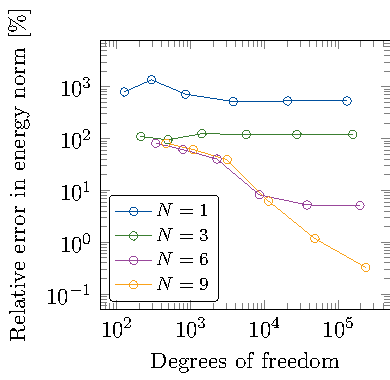
\includegraphics[width=\textwidth]{../../LaTeX/createFigures/TikzFigures/articleIGA_PhD/mockShellConvergence_1}
	\caption{BGC}
	\end{subfigure}%
	\hspace*{0.02\textwidth}%
	\begin{subfigure}{0.49\textwidth}
		\centering
%		\includegraphics[width=\textwidth]{\graphicsFolder/Figure21b}
		\includegraphics[width=\textwidth]{../../LaTeX/createFigures/TikzFigures/articleIGA_PhD/mockShellConvergence_2}
		\caption{BGU}
	\end{subfigure}%
	\par\bigskip
	\par\bigskip
	\begin{subfigure}{0.49\textwidth}
		\centering
%		\includegraphics[width=\textwidth]{\graphicsFolder/Figure21c}
		\includegraphics[width=\textwidth]{../../LaTeX/createFigures/TikzFigures/articleIGA_PhD/mockShellConvergence_3}
		\caption{PGC}
	\end{subfigure}%
	\hspace*{0.02\textwidth}%
	\begin{subfigure}{0.49\textwidth}
		\centering
%		\includegraphics[width=\textwidth]{\graphicsFolder/Figure21d}
		\includegraphics[width=\textwidth]{../../LaTeX/createFigures/TikzFigures/articleIGA_PhD/mockShellConvergence_4}
		\caption{PGU}
	\end{subfigure}%
	\caption{\textbf{Radial pulsation from a mock shell}: Convergence plots for the four infinite element formulations. The relative error in the energy norm (\Cref{Eq2:energyNormFluids}) is plotted against the number of degrees of freedom.}
	\label{Fig2:MS_convergence}
\end{figure}

\begin{figure}
	\begin{subfigure}{0.49\textwidth}
		\centering
%		\includegraphics[width=0.835\textwidth]{\graphicsFolder/Figure22a}
		\includegraphics{../../LaTeX/createFigures/TikzFigures/articleIGA_PhD/mockShellConvergence_5}
		\caption{BGC with the shifted Chebyshev basis}
	\end{subfigure}%
	\hspace*{0.02\textwidth}%
	\begin{subfigure}{0.49\textwidth}
		\centering
%		\includegraphics[width=0.835\textwidth]{\graphicsFolder/Figure22b}
		\includegraphics{../../LaTeX/createFigures/TikzFigures/articleIGA_PhD/mockShellConvergence_6}
		\caption{BGU with the shifted Chebyshev basis}
	\end{subfigure}
	\par\bigskip
	\begin{subfigure}{0.49\textwidth}
		\centering
%		\includegraphics[width=0.835\textwidth]{\graphicsFolder/Figure22c}
		\includegraphics{../../LaTeX/createFigures/TikzFigures/articleIGA_PhD/mockShellConvergence_7}
		\caption{BGC with the Bernstein basis}
	\end{subfigure}%
	\hspace*{0.02\textwidth}%
	\begin{subfigure}{0.49\textwidth}
		\centering
%		\includegraphics[width=0.835\textwidth]{\graphicsFolder/Figure22d}
		\includegraphics{../../LaTeX/createFigures/TikzFigures/articleIGA_PhD/mockShellConvergence_8}
		\caption{BGU with the Bernstein basis}
	\end{subfigure}
	\par\bigskip
	\begin{subfigure}{0.49\textwidth}
		\centering
%		\includegraphics[width=0.835\textwidth]{\graphicsFolder/Figure22e}
		\includegraphics{../../LaTeX/createFigures/TikzFigures/articleIGA_PhD/mockShellConvergence_9}
		\caption{BGC with the Lagrange basis}
	\end{subfigure}%
	\hspace*{0.02\textwidth}%
	\begin{subfigure}{0.49\textwidth}
		\centering
%		\includegraphics[width=0.835\textwidth]{\graphicsFolder/Figure22f}
		\includegraphics{../../LaTeX/createFigures/TikzFigures/articleIGA_PhD/mockShellConvergence_10}
		\caption{BGU with the Lagrange basis}
	\end{subfigure}
	\caption{\textbf{Radial pulsation from a mock shell}: Convergence plots for the BGC and BGU formulations using three different sets of radial shape functions (Chebyshev, Bernstein and Lagrange). The condition number (1-norm condition number estimate provided by \texttt{condest} in \MATLAB) is plotted against the number of degrees of freedom.}
	\label{Fig2:MS_condNumbersB}
\end{figure}


\begin{figure}
	\begin{subfigure}{0.49\textwidth}
		\centering
%		\includegraphics[width=0.835\textwidth]{\graphicsFolder/Figure23a}
		\includegraphics{../../LaTeX/createFigures/TikzFigures/articleIGA_PhD/mockShellConvergence_11}
		\caption{PGC with the shifted Chebyshev basis}
	\end{subfigure}%
	\hspace*{0.02\textwidth}%
	\begin{subfigure}{0.49\textwidth}
		\centering
%		\includegraphics[width=0.835\textwidth]{\graphicsFolder/Figure23b}
		\includegraphics{../../LaTeX/createFigures/TikzFigures/articleIGA_PhD/mockShellConvergence_12}
		\caption{PGU with the shifted Chebyshev basis}
	\end{subfigure}
	\par\bigskip
	\begin{subfigure}{0.49\textwidth}
		\centering
%		\includegraphics[width=0.835\textwidth]{\graphicsFolder/Figure23c}
		\includegraphics{../../LaTeX/createFigures/TikzFigures/articleIGA_PhD/mockShellConvergence_13}
		\caption{PGC with the Bernstein basis}
	\end{subfigure}%
	\hspace*{0.02\textwidth}%
	\begin{subfigure}{0.49\textwidth}
		\centering
%		\includegraphics[width=0.835\textwidth]{\graphicsFolder/Figure23d}
		\includegraphics{../../LaTeX/createFigures/TikzFigures/articleIGA_PhD/mockShellConvergence_14}
		\caption{PGU with the Bernstein basis}
	\end{subfigure}
	\par\bigskip
	\begin{subfigure}{0.49\textwidth}
		\centering
%		\includegraphics[width=0.835\textwidth]{\graphicsFolder/Figure23e}
		\includegraphics{../../LaTeX/createFigures/TikzFigures/articleIGA_PhD/mockShellConvergence_15}
		\caption{PGC with the Lagrange basis}
	\end{subfigure}%
	\hspace*{0.02\textwidth}%
	\begin{subfigure}{0.49\textwidth}
		\centering
%		\includegraphics[width=0.835\textwidth]{\graphicsFolder/Figure23f}
		\includegraphics{../../LaTeX/createFigures/TikzFigures/articleIGA_PhD/mockShellConvergence_16}
		\caption{PGU with the Lagrange basis}
	\end{subfigure}
	\caption{\textbf{Radial pulsation from a mock shell}: Convergence plots for the PGC and PGU formulations using three different sets of radial shape functions (Chebyshev, Bernstein and Lagrange). The condition number (1-norm condition number estimate provided by \texttt{condest} in \MATLAB) is plotted against the number of degrees of freedom.}
	\label{Fig2:MS_condNumbersP}
\end{figure}

It is clear that the choice of basis functions in the infinite elements plays a crucial role for the condition number, and more research is required to find the optimal set of basis functions. Based on the findings in this work, it is recommended to use the BGU formulation alongside the Lagrange basis (in the radial direction) in the infinite elements. However, if larger $N$ is needed for accuracy, the Chebyshev basis is recommended.

\subsection{Stripped BeTSSi submarine}
Finally, we consider the \textit{stripped BeTSSi submarine}\footnote{Based upon the BeTSSi submarine which originates from the BeTSSi workshops~\cite{Gilroy2013bib}.} described in \Cref{Sec2:BeTSSi_description}. 

Let a plane wave, with the direction of incidence given by
\begin{equation}
	\vec{d}_{\mathrm{s}} = -\begin{bmatrix}
		\cos\beta_{\mathrm{s}}\cos\alpha_{\mathrm{s}}\\
		\cos\beta_{\mathrm{s}}\sin\alpha_{\mathrm{s}}\\
		\sin\beta_{\mathrm{s}}
	\end{bmatrix}, \quad\text{where}\quad \alpha_{\mathrm{s}} = \ang{240},\,\beta_{\mathrm{s}} = \ang{0},
\end{equation}
be scattered by this submarine. The CAD model is given in \Cref{Fig2:BC_strippedAndMesh} alongside computational meshes. Again, we shall denote by ${\cal M}_{m,\check{p},\check{k}}^{\textsc{iga}}$, mesh number $m$ with polynomial order $\check{p}$ and continuity $\check{k}$ across element boundaries of the NURBS parametrization. 

\begin{figure}
	\begin{subfigure}{\textwidth}
		\centering
%		\includegraphics[width=0.95\textwidth]{\graphicsFolder/Figure24a}
		\includegraphics[width=0.95\textwidth]{../../graphics/BC/BeTSSi_BC_stripped}
		\caption{CAD model.}
		\label{Fig2:BC_stripped}
	\end{subfigure}
	\par\bigskip
	\par\bigskip
	\begin{subfigure}{\textwidth}
		\centering
%		\includegraphics[width=0.95\textwidth]{\graphicsFolder/Figure24b}
		\includegraphics[width=0.95\textwidth]{../../graphics/BC/mesh1}
		\caption{Surface mesh for mesh ${\cal M}_{1,\check{p},\check{k}}^{\mathrm{IGA}}$}
	\end{subfigure}	
	\par\bigskip
	\par\bigskip
	\begin{subfigure}{\textwidth}
		\centering
%		\includegraphics[width=0.95\textwidth]{\graphicsFolder/Figure24c}
		\includegraphics[width=0.95\textwidth]{../../graphics/BC/mesh2}
		\caption{Surface mesh for mesh ${\cal M}_{2,\check{p},\check{k}}^{\mathrm{IGA}}$.}
	\end{subfigure}	
	\par\bigskip
	\par\bigskip
	\begin{subfigure}{\textwidth}
		\centering
%		\includegraphics[width=0.95\textwidth]{\graphicsFolder/Figure24d}
		\includegraphics[width=0.95\textwidth]{../../graphics/BC/mesh1_eta}
		\caption{Crossection in the $xz$-plane for mesh ${\cal M}_{1,\check{p},\check{k}}^{\mathrm{IGA}}$.}
	\end{subfigure}	
	\par\bigskip
	\par\bigskip
	\begin{subfigure}{\textwidth}
		\centering
%		\includegraphics[width=0.95\textwidth]{\graphicsFolder/Figure24e}
		\includegraphics[width=0.95\textwidth]{../../graphics/BC/mesh2_eta}
		\caption{Crossection in the $xz$-plane for mesh ${\cal M}_{2,\check{p},\check{k}}^{\mathrm{IGA}}$.}
	\end{subfigure}	
	\caption{\textbf{Stripped BeTSSi submarine}: CAD model and meshes used for computations.}
	\label{Fig2:BC_strippedAndMesh}
\end{figure}
The near field at $f=\SI{1000}{Hz}$ is visualized in \Cref{Fig2:BC_NearField}.
\begin{figure}
	\centering    
	\begin{subfigure}[b]{\textwidth}
		\centering
%		\includegraphics[width=\textwidth]{\graphicsFolder/Figure25a}
		\includegraphics[width=\textwidth]{../../LaTeX/createFigures/TikzFigures/articleIGA_PhD/BC_nearField_1}
		\caption{Real part of the incident wave $p_{\mathrm{inc}}(\vec{x})=P_{\mathrm{inc}}\euler^{\imag k\vec{d}_{\mathrm{s}}\cdot \vec{x}}$.}
	\end{subfigure}
	\par\bigskip
	\begin{subfigure}[b]{\textwidth}
		\centering
%		\includegraphics[width=\textwidth]{\graphicsFolder/Figure25b}
		\includegraphics[width=\textwidth]{../../LaTeX/createFigures/TikzFigures/articleIGA_PhD/BC_nearField_2}
		\caption{Real part of the scattered pressure $p(\vec{x})$.}
	\end{subfigure}
	\par\bigskip
	\begin{subfigure}[b]{\textwidth}
		\centering
%		\includegraphics[width=\textwidth]{\graphicsFolder/Figure25c}
		\includegraphics[width=\textwidth]{../../LaTeX/createFigures/TikzFigures/articleIGA_PhD/BC_nearField_3}
		\caption{Real part of the total pressure $p_{\mathrm{tot}}(\vec{x})=p_{\mathrm{inc}}(\vec{x})+p(\vec{x})$.}
	\end{subfigure}
	\par\bigskip
	\begin{subfigure}[b]{\textwidth}
		\centering
%		\includegraphics[width=\textwidth]{\graphicsFolder/Figure25d}
		\includegraphics[width=\textwidth]{../../LaTeX/createFigures/TikzFigures/articleIGA_PhD/BC_nearField_4}
		\caption{Modulus of the total pressure $p_{\mathrm{tot}}(\vec{x})=p_{\mathrm{inc}}(\vec{x})+p(\vec{x})$.}
	\end{subfigure}
	\caption{\textbf{Stripped BeTSSi submarine with SHBC}: The simulation at $f=\SI{1000}{Hz}$ is visualized in the $xy$-plane, and is computed on mesh ${\cal M}_{2,3,2}^{\mathrm{IGA}}$ and the BGU formulation with $N=4$. The numerical evaluations outside the (transparent) prolate ellipsoidal artificial boundary are evaluated with \Cref{Eq2:KirchhoffIntegral}.}
	\label{Fig2:BC_NearField}
\end{figure}
The low frequency problem at $f = \SI{100}{Hz}$ is considered in~\Cref{Fig2:FarField100}. In this case, mesh ${\cal M}_{1,2,1}^{\mathrm{IGA}}$ resolves this frequency, but the solution slightly deviates from the reference solution computed by IGABEM on a fine mesh. The reason for this is that $N$ is too low. Although $N=3$ was enough for engineering precision (below 1\%) in the mock shell example, it does not suffice for the more complicated geometry like the stripped BeTSSi submarine. Consider the relative error for the far field at the well resolved mesh ${\cal M}_{2,3,2}^{\mathrm{IGA}}$. In this case the error will originate from the low resolution (governed by $N$) in the radial direction for the infinite elements. As illustrated in \Cref{Fig2:FarField100error} an order of magnitude in accuracy is gained by increasing $N$. This effect was also observed by the verification test in \Cref{Subsec2:mockShell} applied to the stripped BeTSSi submarine.
\begin{figure}
	\centering    
%	\includegraphics[width=\textwidth]{\graphicsFolder/Figure26}
	\includegraphics[width=\textwidth]{../../LaTeX/createFigures/TikzFigures/articleIGA_PhD/BC_farField100_1}
	\caption{\textbf{Stripped BeTSSi submarine with SHBC}: Computation of target strength (\Cref{Eq2:TS}) at $f=\SI{100}{Hz}$ as a function of the azimuth angle in the spherical coordinate system. The two IGA results (both using $N=3$) are visually indistinguishable meaning that mesh ${\cal M}_{1,2,1}^{\mathrm{IGA}}$ is well resolved for this frequency.}
	\label{Fig2:FarField100}
\end{figure}
\begin{figure}
	\centering    
%	\includegraphics[width=\textwidth]{\graphicsFolder/Figure27}
	\includegraphics[width=\textwidth]{../../LaTeX/createFigures/TikzFigures/articleIGA_PhD/BC_farField100_2}
	\caption{\textbf{Stripped BeTSSi submarine with SHBC}: Computation of the relative error in the far field (\Cref{Eq2:KirchhoffIntegral}) compared to a reference solution at $f=\SI{100}{Hz}$. The computations are done using IGA on mesh ${\cal M}_{2,3,2}^{\mathrm{IGA}}$ using the BGU formulation.}
	\label{Fig2:FarField100error}
\end{figure}
In \Cref{Fig2:FarField} the target strength is plotted for $f=\SI{500}{Hz}$ and $f=\SI{1000}{Hz}$. A reference solution (using IGABEM) is added for the $f=\SI{500}{Hz}$ case, and illustrates again the pollution of low $N$. The IGA mesh 1 resolves the frequency $f=\SI{500}{Hz}$ quite well using only about 5 elements per wavelength. This corresponds to about 5 dofs per wavelength in each dimensional direction compared to the classical 10-12 dofs per wavelength needed for FEM methods.
\begin{figure}
	\centering    
	\begin{subfigure}[b]{\textwidth}
		\centering
%		\includegraphics[width=\textwidth]{\graphicsFolder/Figure28a}
		\includegraphics[width=\textwidth]{../../LaTeX/createFigures/TikzFigures/articleIGA_PhD/BC_farField_1}
		\caption{$f=\SI{500}{Hz}$}
	\end{subfigure}
	\par\bigskip
	\par\bigskip
	\begin{subfigure}[b]{\textwidth}
		\centering
%		\includegraphics[width=\textwidth]{\graphicsFolder/Figure28b}
		\includegraphics[width=\textwidth]{../../LaTeX/createFigures/TikzFigures/articleIGA_PhD/BC_farField_2}
		\caption{$f=\SI{1000}{Hz}$}
	\end{subfigure}
	\caption{\textbf{Stripped BeTSSi submarine with SHBC}: Computation of target strength (\Cref{Eq2:TS}) as a function of the azimuth angle in the spherical coordinate system. The numerical evaluations are evaluated with \Cref{Eq2:TS}.}
	\label{Fig2:FarField}
\end{figure}
